\documentclass[12pt,a4paper]{beamer}
\usetheme{Madrid}
\usepackage{tikz}
\usepackage{amsmath}
\usepackage{graphics}
\author{\bf{Devendra Raj Upadhyay}}
\institute{CDP, TU}
\logo{
\includegraphics[height=1cm]{logo.eps}}
\title[ISM \& AGB Star]{\Large\bf{INTERACTION BETWEEN AMBIENT INTERSTELLAR MEDIUM AND ASYMPTOTIC GIANT BRANCH STARS AT LATITUDE
32.47$^{\circ}$ $\&$ 40.67$^{\circ}$0 Proposed}}
\subtitle{Dissertation}
\date{\today}
\begin{document}
\begin{frame}
\begin{center}
\Large\bf{\color{blue}``INTERACTION BETWEEN AMBIENT INTERSTELLAR MEDIUM AND ASYMPTOTIC GIANT BRANCH STARS AT LATITUDE
32.47$^{\circ}$ $\&$ 40.67$^{\circ}$''}\\[1cm]
Dissertation\\[1cm]
\bf{Devendra Raj Upadhyay}
{\color{blue}\\Central Department of Physics\\Institute of Science \& Technology\\Tribhuvan University, Kathmandu, Nepal}\\
\end{center}
\end{frame}
\begin{frame}{Outline}
\begin{itemize}
\item<1-> {Why ISM \& AGB?}
\item<1-> Introduction
\item<1-> Theory
\item<1-> Region of Interest
\item<1-> Methodology
\item<1-> Results and Discussions
\item<1-> Conclusions
\item<1-> Acknowledgement
\item<1-> References
\item<1-> Questions !!!
\end{itemize}
\end{frame}

\begin{frame}
\begin{center}
\Large\bf\color{red}{Why ISM \& AGB?}
\end{center}
\end{frame}


\begin{frame}{Why ISM \& AGB ?}
\begin{figure}[h]
\vspace{0.0cm} \centering
  \includegraphics[width =6cm]{Shock}\cite{10}
\end{figure}
\end{frame}

\begin{frame}{Why ISM \& AGB ? (Cont...)}
 \begin{figure}[h]
 \begin{block}{\centering\textbf{Hertzsprung $-$ Russell diagram \vspace*{.25cm}}}
\vspace{0.0cm} \centering
\includegraphics[width=6cm]{HR.eps}\cite{26}
\end{block}
\end{figure}
\end{frame}

\begin{frame}
\begin{center}
\Large\bf\color{red}{Introduction}
\end{center}
\end{frame}

\begin{frame}{Introduction}
\begin{block}{\centering\textbf{Motivations \vspace*{.25cm}}}
\begin{itemize}
\item  It is believed that the shaping of infrared dust structure
has a close relation with the inhomogeneous Interstellar Medium
(ISM). The violent stellar phenomena lead inhomogeneity in the
ISM. We are interested to perform a multi wavelength study in the
far infrared emission region. This may reveal the presence and
role of hot phenomena (X-rays, gamma rays, etc) in the shaping
process. \item  We are interested to correlate inhomogeneous
phenomena occur in ISM as well as C-rich AGB wind with Green
Function Method.
 \item Asymmetry mass ejection during the AGB phase was concluded
 by Zijlstra \& Weinberger (2002), Aryal \& Weinberger (2006), Aryal, Rajbahak \& Weinberger
(2009), Aryal, Rajbahak \& Weinberger (2010) by studying dust
structures around planetary nebula.\cite{6,7,8,9}.
\end{itemize}
\end{block}
\end{frame}

\begin{frame}{Introduction}
\begin{block}{\centering\textbf{Motivations \vspace*{.25cm} (Cont...)}}
\begin{itemize}
\item Search for any stellar
objects which might be capable of shaping an interstellar cloud of
small or moderate mass; such an object should be located at or
around the extended emission.\cite{9} With SIMBAD, we intend to
investigate discrete sources in the field of the infrared emission
that might be responsible for cavity formation near AGB star.
\end{itemize}
\end{block}
\end{frame}


\begin{frame}{Introduction}
\begin{block}{\centering\textbf{Objectives \vspace*{.25cm}}}
\begin{itemize}
\item We want to investigate the new isolated cavity structure including cavity in
 IRAS maps by performing a systematic search in all wavelength
 band in the IRAS survey of our C-rich AGB star catalogue.
\item We want to investigate the dust color temperature, mass
 profile, outflow velocity and associated energy of the structure.
\item To know the model of cavity formation due to AGB wind, we
study the flux density variation along the major diameter, minor
diameter and along the line joining the region of minimum
temperature and minimum flux.
\item We are also interested to
estimate Shock nature, i.e., C-shock and J-shock ejected by AGB
wind. By knowing inhomogeneous nature of medium we try to
correlate or interpret in term of Green's function technique.
\end{itemize}
\end{block}
\end{frame}

 \begin{frame}
\begin{center}
\Large\bf\color{red}{Theory}
\end{center}
\end{frame}




\begin{frame}{Theory (Cont...)}
\begin{block}{\centering\textbf{Mass Estimation \vspace*{.05cm}}}
\begin{itemize}
\begin{equation}
 M_{dust} = \frac{4}{{3}}\frac{a\rho}{{Q_{\nu}}}\bigg[\frac{S_{\nu}D^{2}}{{B(\nu, T)}}\bigg]
\end{equation}
Where,
$a$ = weighted grain size,
$\rho$ = grain density,
$ Q_{\nu}$ = grain emissivity,
$D$ = the distance to the Star,
$ S_{\nu}$ = f $\times$ MJy/Sr $\times$ 5.288 $\times$ 10$^{-9}$
\cite{40}\end{itemize}
\end{block}



\begin{frame}{Theory (Cont...)}
\begin{block}{\centering\textbf{For 100 $\mu$m emitter \vspace*{.05cm}}}
\begin{itemize}
a = 0.1 $\mu$m, $\rho$ = grain density =
1000 kg m$^{−3}$ , Q$_{\nu}$ = grain emissivity = 0.0010 (for 100 $\mu$m), Q$_{\nu}$ =
grain emissivity = 0.0046 (for 60 $\mu$m) (Young $et$ $al.$
(1989)\cite{39}. $ S_{\nu}$ = f $\times$ MJy/Sr $\times$ 5.288 $\times$ 10$^{-9}$
where, 1 MJy/Sr = 1 $\times 10^{-20}$ kg s$^{-2}$ and f = relative
flux density measured from the Groningen IRAS image.\cite{40, 41}
\begin{equation}\label{9}
    M_{dust} = 0.40\bigg[\frac{S_{\nu}D^{2}}{{B(\nu, T)}}\bigg]
\end{equation}
\end{itemize}
\end{block}
\end{frame}

\begin{frame}{Theory (Cont...)}
\begin{block}{\centering\textbf{Planck's Function \vspace*{.05cm}}}
\begin{itemize}
\begin{equation}\label{10}
    B(\nu, T) = \frac{2h\nu^{3}}{{c^{2}}}\bigg[\frac{1}{exp^(\frac{h\nu}{KT})-1}\bigg]
\end{equation}
Where,
$h$ = Planck's constant,
$c$ = velocity of light,
${\nu}$ = frequency at which the emission is observed,
$T$ = Temperature
\end{itemize}
\end{block}
\end{frame}

\begin{frame}{Theory (Cont...)}
\begin{block}{\centering\textbf{Out flow \cite{42, 43} \vspace*{.05cm}}}
\begin{itemize}
\begin{equation}
u_{out}^{2} = (\frac{2}{\gamma - 1})C_{s}^{2}(R_{c}) + (\Gamma
-1)u_{esc}^{2}(R_{c})
\end{equation}
Where, where $ u_{esc} $ = the escape speed, $ c_{s}$ = the sound,
speed, $ R_{c} $ =  the condensation radius, and $ \gamma $ = the
polytropic index, $\Gamma$ =
$\frac{\kappa{L_\star}}{4{\pi}c{G}{M_{\star}}}$  and
$\kappa_{crit}$ = $\frac{4{\pi}c{G}{M_{\star}}}{{L_\star}}$
\end{itemize}
\end{block}
\end{frame}



\begin{frame}{Theory (Cont...)}
\begin{block}{\centering\textbf{Typical global properties of AGB stars.\cite{45}}}
 \begin{table}[h]
$$
\begin{array}{p{0.3\linewidth}ccc}
            \hline
            \hline
            \noalign{\smallskip}
            Parameter & Value Range \\
            \noalign{\smallskip}
            \hline
            \hline
            \noalign{\smallskip}
Mass, $M$    &   0.8 - 8 M_{\odot}\\
Radius, $R$  &   200 - 600 R_{\odot}, (1 - 3 AU)\\
Temperature, $T_{eff}$   &   3500- 3500 K\\
Luminosity, $M_{bol}$, (L)  &   {-3.6} to {-7.1}  mag, (10^{3} - 10^{4}L_{\odot})\\
Mass loss rate, $\dot{M}$   &   10^{-8} - 10^{-4} M_{\odot} yr^{-1}\\
Variable Period, $P$   &  30 - 2800 days\\
AGB timescale, $\tau_{AGB}$   &  10^5 -5\times10^{6} yrs \\
             \noalign{\smallskip}
            \hline
            \hline
         \end{array}
     $$
\end{table}
\end{block}
\end{frame}

\begin{frame}{Theory (Cont...)}
\begin{block}{\centering\textbf{Energy Estimation}}
\begin{equation}
    E = \frac{1}{2}M_{deficit}u_{out}^{2}
\end{equation}
\end{block}
\end{frame}

\begin{frame}
\begin{center}
\Large\bf\color{red}{Region of Interest}
\end{center}
\end{frame}

\begin{frame}{Region of Interest}
\begin{block}{\centering\textbf{IRAS \cite{32,33} \vspace*{.5cm}}}
\begin{itemize}
IRAS was a joint project of the US, UK and the Netherlands. The
IRAS mission performed an unbiased, sensitive all sky survey at
12, 25, 60 and 100 $\mu$m. The satellite design and survey
strategy were optimized for maximally reliable detection of point
sources. For ten months in 1983, the Infrared Astronomical
Satellite (IRAS) scanned more than 96 $\%$ of the sky.
 \begin{figure}[h]
\vspace{0.0cm} \centering
\includegraphics[width=5cm]{IRAS1}
\includegraphics[width=5cm]{IRAS}
\end{figure}
\end{itemize}
\end{block}
\end{frame}
\begin{frame}{Region of Interest (Cont...)}
\begin{block}{\centering\textbf{Different Satellites \vspace*{.5cm}}}
\begin{figure}[h]
\vspace{0.0cm} \centering
\includegraphics[width=10cm]{5.eps}
\end{figure}
\end{block}
\end{frame}

\begin{frame}{Region of Interest (Cont...)}
\begin{block}{\centering\textbf{Different Regions \vspace*{.5cm}}}
\begin{figure}[h]
\vspace{0.0cm} \centering
\includegraphics[width=10cm]{n.eps}
\end{figure}
\end{block}
\end{frame}

\begin{frame}{Region of Interest (Cont...)}
\begin{block}{\centering\textbf{Different Surveys \vspace*{.5cm}}}
\begin{figure}[h]
\vspace{0.0cm} \centering
\includegraphics[width=8cm]{pq.eps}
\end{figure}
\end{block}
\end{frame}

\begin{frame}{Region of Interest (Cont...)}
\begin{block}{\centering\textbf{Different Surveys \vspace*{.5cm}}}
\begin{figure}[h]
\vspace{0.0cm} \centering
\includegraphics[width=10cm]{3.eps}
\end{figure}
\end{block}
\end{frame}

\begin{frame}{Region of Interest (Cont...)}
\begin{block}{\centering\textbf{Infrared Universe \vspace*{.5cm}}}
\begin{figure}[h]
\vspace{0.0cm} \centering
\includegraphics[width=10cm]{8.eps}
\end{figure}
\end{block}
\end{frame}

\begin{frame}{Region of Interest (Cont...)}
\begin{block}{\centering\textbf{Infrared Universe \vspace*{.5cm}}}
\begin{figure}[h]
\vspace{0.0cm} \centering
\includegraphics[width=8cm]{p.eps}
\end{figure}
\end{block}
\end{frame}

\begin{frame}{Region of Interest (Cont...)}
\begin{block}{\centering\textbf{Infrared World \vspace*{.5cm}}}
\begin{figure}[h]
\vspace{0.0cm} \centering
\includegraphics[width=10cm]{6.eps}
\end{figure}
\end{block}
\end{frame}

\begin{frame}{Region of Interest (Cont...)}
\begin{block}{\centering\textbf{Infrared World \vspace*{.5cm}}}
\begin{figure}[h]
\vspace{0.0cm} \centering
\includegraphics[width=12cm]{7.eps}
\end{figure}
\end{block}
\end{frame}


\begin{frame}{Region of Interest (Cont...)}
\begin{block}{\centering\textbf{IRAS with Different Wavelengths \vspace*{.5cm}}}
\begin{figure}[h]
\vspace{0.0cm} \centering
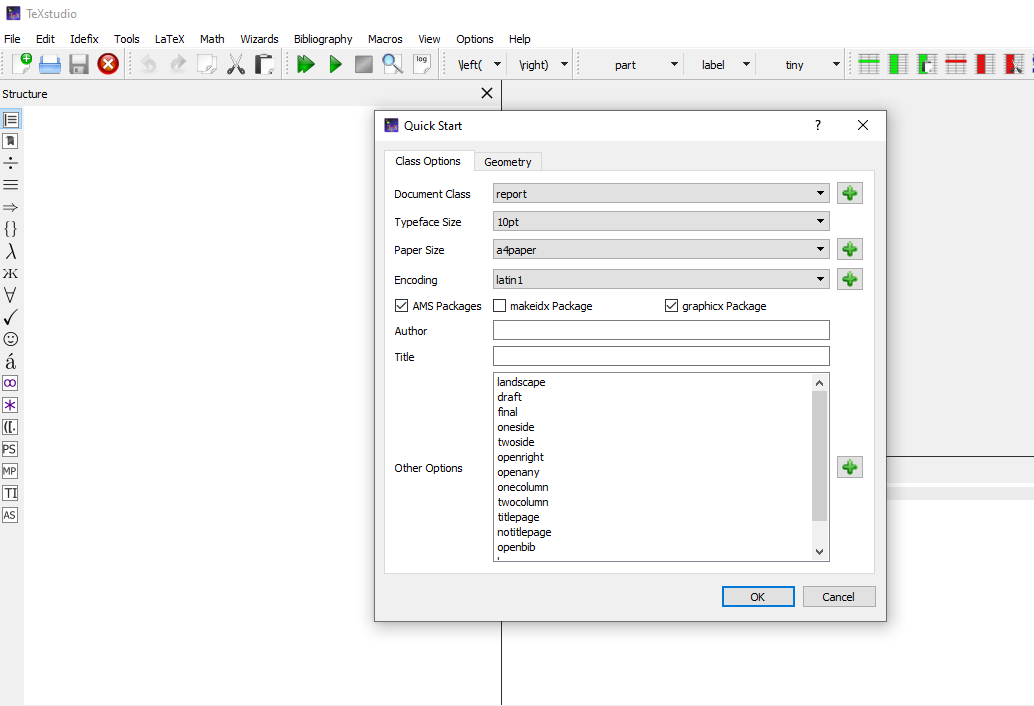
\includegraphics[width=10cm]{1.eps}
\end{figure}
\end{block}
\end{frame}



\begin{frame}{Region of Interest (Cont...)}
\begin{block}{\centering\textbf{1168 C-rich AGB Stars \vspace*{.5cm}}}
 Suh \& Kwon 2011 presented a catalog of AGB stars for 3003 O-rich, 1168 C-rich, 362 S-type and 35 silicate carbon stars in our Galaxy which is a revised version of the catalog of AGB stars by Suh \& Kwon (2009)
\begin{figure}[h]
\vspace{0.0cm} \centering
\includegraphics[width=8cm]{skyscan}
\end{figure}
\end{block}
\end{frame}



\begin{frame}{Region of Interest (Cont...)}
\begin{block}{\centering\textbf{250 C-rich AGB Stars \vspace*{.5cm}}}
\begin{itemize}
\begin{figure}[h]
\vspace{0.0cm} \centering
\includegraphics[width=6cm]{agb250}
\end{figure}
\end{itemize}
\end{block}
\end{frame}

\begin{frame}{Region of Interest (Cont...)}
\begin{block}{\centering\textbf{Targeted $\&$ Near by  C-rich AGB Stars \vspace*{.5cm}}}
\begin{itemize}
\begin{figure}[h]
\vspace{0.0cm} \centering
\includegraphics[width=6cm]{agb}
\end{figure}
\end{itemize}
\end{block}
\end{frame}

\begin{frame}{Region of Interest (Cont...)}
\begin{block}{\centering\textbf{Inspection in  Skyview Virtual observatory\cite{34} \vspace*{.5cm}}}
\begin{itemize}
\begin{figure}[h]
Coordinate: J2000 \\
Projection: Gnomonic(Tan)\\
Image size (pixel): 500$\times$500\\
Image Size (degrees): 0.5$\times$0.5, 0.6$\times$0.6 and 0.7$\times$0.7\\
Brightness Scaling: Histogram Equilization(HistEq)\\
Color Table: Stern Special\\
Sampler:    NN Sampler\\
Provenance: NASA IPAC/Jet Propulsion Laboratory\\
Copyright: Public Domain\\
\end{figure}
\end{itemize}
\end{block}
\end{frame}

\begin{frame}{Region of Interest (Cont...)}
\begin{block}{\centering\textbf{AGB Star 9 (J2000.0: 00 42 13.37 +53 02 17.4) \cite{34,35} \vspace*{.5cm}}}
\begin{itemize}
\begin{figure}
\vspace{0.0cm} \centering
\includegraphics[width=2.5cm]{100m}
\includegraphics[width=2.5cm]{60m}
\includegraphics[width=2.5cm]{IRAS25micron}
\includegraphics[width=2.5cm]{IRAS12micron}
\end{figure}
\end{itemize}
\end{block}
\end{frame}

 \begin{frame}{Region of Interest (Cont...)}
\begin{block}{\centering\textbf{AGB Star 161 (J2000.0: 05 37 02.52 -08 25 46.8)\cite{34,35} \vspace*{.5cm}}}
\begin{itemize}
\begin{figure}[h]
\vspace{0.0cm} \centering
\includegraphics[width=2.5cm]{100m161}
\includegraphics[width=2.5cm]{60m161}
\includegraphics[width=2.5cm]{25m161}
\includegraphics[width=2.5cm]{12m161}
\end{figure}
\end{itemize}
\end{block}
\end{frame}

        \begin{frame}{Region of Interest (Cont...)}
\begin{block}{\centering\textbf{SIMBAD Result Objects found within 0.1 degree radius \cite{35}}}
\begin {table}[h]
$$
\begin{array}{p{0.1\linewidth}cccccc}
            \hline
            \hline
            \noalign{\smallskip}
            Identifier & {\rm Dist} & {\rm Type} & {\rm R.A.(J2000)} & {\rm Dec.(J2000)} & {\rm Refrences}\\
            &{\rm(asec)}&&&&{\rm 1850 - 2015}\\
            \noalign{\smallskip}
            \hline
            \hline
            \noalign{\smallskip}
   B3 0013+457     &   98.45   &   Rad  &   00 16 09        &   +46 0 0.5       &     0   \\
   TYC 3247-1413-1 &   146.85  &   *    &   00 15 49.316    &   +45 58 24.27    &     0   \\
   TYC 3247-1349-1 &   190.65  &   *    &   00 16 18.1315   &   +45 59 34.509   &     0   \\
   TYC 3247-1487-1 &   335.98  &   *    &   00 15 31.745    &   +46 02 42.09    &     0   \\
             \noalign{\smallskip}
            \hline
            \hline
         \end{array}
     $$
       \end{table}
\end{block}
\end{frame}

\begin{frame}{Region of Interest (Cont...)}
\begin{block}{\centering\textbf{SIMBAD Result Objects found within 0.1 degree radius \cite{35}}}
\begin {table}[h]
$$
\begin{array}{p{0.1\linewidth}cccccc}
            \hline
            \hline
            \noalign{\smallskip}
            Identifier & {\rm Dist} & {\rm Type} & {\rm R.A.(J2000)} & {\rm Dec.(J2000)} & {\rm Refrences}\\
            &{\rm(asec)}&&&&{\rm 1850 - 2015}\\
            \noalign{\smallskip}
            \hline
            \hline
            \noalign{\smallskip}
            TYC 8-222-1             &   231.02  &   *   &   00 19 53.958      &  +06 03 56.30    &     0   \\
            2MASX J00202779 +0600189 &   340.28  &   G   &   00 20 27.799      &  +06 00 18.95    &     0   \\
             \noalign{\smallskip}
            \hline
            \hline
         \end{array}
     $$
        \end{table}
\end{block}
\end{frame}

\begin{frame}{Region of Interest (Cont...)}
\begin{block}{\centering\textbf{ R.A.(J2000) =$04^{\rm h}46^{\rm m}13.84^{\rm s}$,
Dec.(J2000) = +32$^{\circ}$31${'}$39.6${''}$,  AGB Star No. 111 \cite{34,35} \vspace*{.5cm}}}
\begin{itemize}
\begin{figure}[h]
\vspace{0.0cm} \centering
\includegraphics[width=2.5cm]{100m111}
\includegraphics[width=2.5cm]{60m111}
\includegraphics[width=2.5cm]{25m111}
\includegraphics[width=2.5cm]{12m111}
\end{figure}
\end{itemize}
\end{block}
\end{frame}


\begin{frame}{Region of Interest (Cont...)}
\begin{block}{\centering\textbf{ R.A.(J2000) =  $05^{\rm
h}05^{\rm m} 59.58^{\rm s}$  Dec.(J2000) = +40$^{\circ}$40${'}$33.4${''}$ AGB Star No. 129 \cite{34,35}\vspace*{.5cm}}}
\begin{itemize}
\begin{figure}[h]
\vspace{0.0cm} \centering
\includegraphics[width=2.5cm]{100m129}
\includegraphics[width=2.5cm]{60m129}
\includegraphics[width=2.5cm]{25m129}
\includegraphics[width=2.5cm]{12m129}
\end{figure}
\end{itemize}
\end{block}
\end{frame}

\begin{frame}
\begin{center}
\Large\bf\color{red}{Methodology}
\end{center}
\end{frame}

\begin{frame}{Methodology}
\begin{block}{\centering\textbf{Data Reduction\\ \vspace*{.5cm}}}
\begin{itemize}
\item \textbf{FITS}
\item \textbf{Aladin v2.5}
\item \textbf{Origin5}
\item \textbf{Computational programs}
\item \textbf{Aladin v8.0}
\end{itemize}
\end{block}
\end{frame}


\begin{frame}{Methodology}
\begin{block}{\centering\textbf{111 Contour Map \vspace*{.5cm}}}
\begin{itemize}
\begin{figure}[h]
\vspace{0.0cm} \centering
\includegraphics[width=5cm]{mc100111}
\includegraphics[width=5cm]{mc60}
\end{figure}
\end{itemize}
\end{block}
\end{frame}

\begin{frame}{Methodology (Cont...)}
\begin{block}{\centering\textbf{129 Contour Map \vspace*{.5cm}}}
\begin{itemize}
\begin{figure}[h]
\vspace{0.0cm} \centering
\includegraphics[width=5cm]{mc1129}
\includegraphics[width=5cm]{mc6129}
\end{figure}
\end{itemize}
\end{block}
\end{frame}


\begin{frame}
\begin{center}
\Large\bf\color{red}{Result \& Discussion}
\end{center}
\end{frame}

\begin{frame}{Result \& Discussion}
\begin{block}{\centering\textbf{Major (AB), Minor (CD) diameters $\&$ Line passes though S$_{\nu}_{mini}$ and T$_{mini}$ (EF) \vspace*{.05cm}}}
\begin{itemize}
\begin{figure}[h]
\vspace{0.0cm} \centering
\includegraphics[width=5cm]{MMM_111}
\includegraphics[width=5cm]{129MMM}
\end{figure}
\end{itemize}
\end{block}
\end{frame}


\begin{frame}{Result \& Discussion (Cont...)}
\begin{block}{\centering\textbf{Flux Density Variation along AB \vspace*{.05cm}}}
\begin{itemize}
\begin{figure}[h]
\vspace{0.0cm} \centering
\includegraphics[width=5cm]{111dVsSvMajor}
\includegraphics[width=5cm]{dVsSvmajor129}
\begin{equation*}\label{LB}
\begin{array}{l}
S_{\nu} = 13.6 - 37.9d + 93.6d^{2} - 194.3d^{3} + 195.2d^{4} - 65.2d^{5}
\\
\\
S_{\nu} = 8.9 - 2.5d + 6.2d^2 - 9.1d^{3} + 6.9d^{4} - 1.9d^{5}
\end{array}
\end{equation*}

\end{figure}
\end{itemize}
\end{block}
\end{frame}

\begin{frame}{Result \& Discussion (Cont...)}
\begin{block}{\centering\textbf{Flux Density Variation along CD \vspace*{.05cm}}}
\begin{itemize}
\begin{figure}[h]
\vspace{0.0cm} \centering
\includegraphics[width=5cm]{dVsSvminor111}
\includegraphics[width=5cm]{dVsSvMinor129}
\end{figure}
\begin{equation*}\label{LB}
\begin{array}{l}
S_{\nu} = 17.9 - 173.4d + 936.4d^{2} - 2316.4d^{3} + 2533.1d^{4} - 989.0d^{5}
\\
\\
S_{\nu} = 9.2 - 7.5d + 27.2d^{2} - 50.4d^{3} + 47.6d^{4} - 17.6d^{5}
\end{array}
\end{equation*}
\end{itemize}
\end{block}
\end{frame}

\begin{frame}{Result \& Discussion (Cont...)}
\begin{block}{\centering\textbf{Flux Density Variation along EF \vspace*{.05cm}}}
\begin{itemize}
\begin{figure}[h]
\vspace{0.0cm} \centering
\includegraphics[width=5cm]{dVsSvminiT111}
\includegraphics[width=5cm]{dVsSvminiT129}
\end{figure}
\begin{equation*}\label{LB}
\begin{array}{l}
S{\nu}=12.6 - 17.1d - 182.0d^{2} + 1092.3d^{3} - 2303.2d^{4} + 2067.3d^{5}\\ - 662.5d^{6}
\\
\\
S_{\nu} = 8.9 - 7.1d + 63.9d^{2} - 292.0d^{3} + 698.4d^{4} - 896.9d^{5}\\ +585.9d^{6} - 153.0d^{7}
\end{array}
\end{equation*}
\end{itemize}
\end{block}
\end{frame}

\begin{frame}{Result \& Discussion (Cont...)}
\begin{block}{\centering\textbf{Dust Color Temperature Variation along AB \vspace*{.05cm}}}
\begin{itemize}
\begin{figure}[h]
\vspace{0.0cm} \centering
\includegraphics[width=5cm]{dVsTMajor111}
\includegraphics[width=5cm]{dVsTmajor129}
\end{figure}
\begin{equation*}\label{LB}
\begin{array}{l}
T = 21.0 + 70.5d - 256.7d^{2} - 482.8d^{3} + 3842.1d^{4}\\ - 6667.8d^{5} + 4668.3d^{6} - 1169.6d^{7}
\\
\\
T = 17.1 + 30.1d - 193.5d^{2} + 575.3d^{3} - 906.3d^{4}\\ + 779.6d^{5} - 345.5d^{6} + 61.7d^{7}
\end{array}
\end{equation*}
\end{itemize}
\end{block}
\end{frame}


\begin{frame}{Result \& Discussion (Cont...)}
\begin{block}{\centering\textbf{Dust Color Temperature Variation along CD \vspace*{.05cm}}}
\begin{itemize}
\begin{figure}[h]
\vspace{0.0cm} \centering
\includegraphics[width=5cm]{dVsTminor111}
\includegraphics[width=5cm]{dVsTminor129}
\end{figure}
\begin{equation*}\label{LB}
\begin{array}{l}
T = -14.8 + 725.5d-4355.7d^{2} + 11578.7d^{3} - 13694.0d^{4}\\ + 5866.3d^{5}
\\
\\
T = 54.7 - 570.8d+3201.3d^{2} - 8676.3d^{3} + 12335.9d^{4}\\ - 8862.2d^{5} + 2538.3d^{6}
\end{array}
\end{equation*}
\end{itemize}
\end{block}
\end{frame}


\begin{frame}{Result \& Discussion (Cont...)}
\begin{block}{\centering\textbf{Dust Color Temperature Variation along EF \vspace*{.05cm}}}
\begin{itemize}
\begin{figure}[h]
\vspace{0.0cm} \centering
\includegraphics[width=5cm]{dVsTmini111}
\includegraphics[width=5cm]{dVsTminiT129}
\end{figure}
\begin{equation*}\label{LB}
\begin{array}{l}
T = 73.1 - 1240.0d + 10234.0d^{2} - 39728.9d^{3} + 82197.7d^{4}\\ - 926323.0d^{5} + 53497.3d^{6} - 12377.3d^{7}
\\
\\
T = 18.4+7.2d-57.8d^{2} + 169.2d^{3} - 191.9d^{4}\\ + 21.4d^{5} + 101.6d^{6} - 49.4d^{7}
\end{array}
\end{equation*}
\end{itemize}
\end{block}
\end{frame}

\begin{frame}{Result \& Discussion (Cont...)}
\begin{block}{\centering\textbf{Dust Mass Estimation of Outer \& Inner Circle \vspace*{.5cm}}}
\begin{itemize}
\begin{figure}[h]
\vspace{0.0cm} \centering
\includegraphics[width=5cm]{111}
\includegraphics[width=5cm]{129}
\end{figure}
\end{itemize}
\end{block}
\end{frame}

\begin{frame}{Result \& Discussion (Cont...)}
\begin{block}{\centering\textbf{Sum, Average, and mass per Pixel of
region of Interest \vspace*{.05cm}}}
\begin{itemize}
\begin{table}
$$
\begin{array}{p{0.15\linewidth}cccc}
            \hline
            \hline
            \noalign{\smallskip}
            Region &{\rm Total\,Mass}&{\rm Average\, Mass}&{\rm Average\, Mass\, Difference}\\
            &{\rm(kg)}&{\rm\,(Kg)}&{\rm\,(Kg)} \\
            \noalign{\smallskip}
            \hline
            \hline
            \noalign{\smallskip}
                  Inner Circle (I)  &  3.182\times10^{25}      &     6.770\times10^{23}     &  \\
                   Outer Circle (I) &  1.205\times10^{26}      &     2.490\times10^{24}     & 1.810\times10^{24}\\
                   Inner Circle (II) &  1.087\times10^{27}      &     5.177\times10^{25}    &   \\
                   Outer Circle (II) &  2.587\times10^{27}      &     1.000\times10^{26}     & 4.656\times10^{25} \\
             \noalign{\smallskip}
            \hline
            \hline
         \end{array}
     $$
\end{table}
\end{itemize}
\end{block}
\end{frame}


\begin{frame}{Result \& Discussion (Cont...)}
\begin{block}{\centering\textbf{AGB outflow \vspace*{.05cm}}}
\begin{itemize}
\begin{table}
\begin{array}{p{0.3\linewidth}cccc}
            \hline
            \hline
            \noalign{\smallskip}
            Region &{\rm c_{s}\,}&{\rm u_{esc}\,}&{u_{out}\,}\\
            &{\rm(ms^{-1})}&{\rm\,(ms^{-1})}&{\rm\,(ms^{-1})} \\
            \noalign{\smallskip}
            \hline
            \hline
            \noalign{\smallskip}
                  Inner Circle (I)  & 6.486      &     0.532     & 12.962\\
                  Inner Circle (II)  & 5.567     &     3.146     & 10.710\\
             \noalign{\smallskip}
            \hline
            \hline
         \end{array}
     $$
\end{table}
\end{itemize}
\end{block}
\end{frame}


\begin{frame}{Result \& Discussion (Cont...)}
\begin{block}{\centering\textbf{Energy Estimation \vspace*{.05cm}}}
\begin{itemize}
 \begin{table}[h]
$$
\begin{array}{p{0.3\linewidth}cccc}
            \hline
            \hline
            \noalign{\smallskip}
            Region &{\rm M_{deficit}\,}&{\rm u_{out}\,}&{E\,}\\
            &{(Kg)}&{\rm\,(ms^{-1})}&{(J)} \\
            \noalign{\smallskip}
            \hline
            \hline
            \noalign{\smallskip}
                  Candidate I        &    1.810\times10^{24}  &   12.962 & 1.173\times^{25}\\
                  Candidate II       &    4.8232\times10^{27} &  10.710 & 2.766\times10^{27}\\
             \noalign{\smallskip}
            \hline
            \hline
         \end{array}
     $$
\end{table}
\end{itemize}
\end{block}
\end{frame}

\begin{frame}{Result \& Discussion   (Cont...)}
\begin{block}{\centering\textbf{Size of the Structure \vspace*{.05cm}}}
\begin{itemize}
 \begin {table}[h]
$$
\begin{array}{p{0.1\linewidth}cccccc}
            \hline
            \hline
            \noalign{\smallskip}
            Contour&{\rm Major\,diameter}&{\rm Minor\,diameter}\\
            & {\rm (pc)}&{\rm (pc)}\\
            \noalign{\smallskip}
            \hline
            \noalign{\smallskip}
            41 & 1.354 & 0.971\\
            52 & 1.424 & 0.925\\
             \noalign{\smallskip}
            \hline
            \hline
         \end{array}
     $$
        \end{table}
\end{itemize}
\end{block}
\end{frame}




        \begin{frame}
\begin{center}
\Large\bf\color{red}{Conclusions}
\end{center}
\end{frame}



\begin{frame}{Conclusion}
\begin{itemize}
\item The  the size of the structure are 1.354 pc $\times$0.971 pc
for candidate I and  1.424 pc $\times$ 0.925 pc for candidate II
where, major and minor diameter is found to be 1.354 pc and 0.971
pc for candidate I and that of candidate II are 1.424 pc and 0.925
pc respectively. \item The minimum flux region is found to be
located at center of lower part, at R.A.(J2000) = $04^{\rm
h}46^{\rm m}13.84^{\rm s}$, Dec.(J2000) =
+32$^{\circ}$31${'}$39.6${''}$ for candidate I and $05^{\rm
h}05^{\rm m}59.58^{\rm s}$, +40$^{\circ}$40${'}$33.4${''}$ for
Candidate II respectively.
 \item A study of distance versus flux density, temperature
variation shows a prominent condensation of dust at 100 $\mu$m
image and Gaussian-like distribution is observed along major and
minor diameters of the structure. In addition, similar
Gaussian-like distribution is found along line joining the minima
and the lower temperature region. Gaussian-like distribution
suggests that the cavity structure is less disturbed from the
external factors, i.e., possibility symmetric phenomena.

\end{itemize}
\end{frame}



\begin{frame}{Conclusion (Cont...)}
\begin{itemize}
\item A
study of outflow suggests that the outflow velocity of structure
is not uniform and not regularly shaped. \item The dust color
temperature is found to lie in the range 21.65 K to 35.64 K for
candidate I and 18.51 K to 19.29 K, with an offset of about 14 K
for candidate I and 0.8 K for candidate II. An offset 14 K
suggests that the AGB is hot in the early stage. Now AGB in late
AGB stage. We expect deviation from symmetrical outflow, i.e., AGB
wind probably prefer polytropic behaviour implies bipolar type
wind. Where as the offset 0.8 K for candidate II suggests that the
AGB is in symmetric AGB phase, i.e., early AGB stage.
\item The
total mass of the dust in the cavity structure is found about
5.93$\times$10$^{25}$ Kg (0.00003 M$_{\odot}$) for candidate I and
1.95$\times$10$^{27}$ Kg (0.001 M$_{\odot}$) for candidate II.
\end{itemize}
\end{frame}


\begin{frame}{Conclusion   (Cont...)}
\begin{itemize}
\item The outflow nature was determined by using sound speed,
escape velocity, mass of dissipation from symmetrical cavity like
structure with the help of these parameter we obtained energy of
dissipation as 1.17$\times$10$^{25}$ J and 2.77 $\times$ 10$^{27}$
J for candidate I and II respectively which suggest that the
energy of the order 10$^{25}$ and 10$^{27}$ Joules falls with in
the limit of AGB wind energy.
\end{itemize}
\end{frame}

\begin{frame}
\begin{center}
\Large\bf\color{red}{Presentations}
\end{center}
\end{frame}
\begin{frame}{Presentations}
\begin{itemize}
\item \textbf{Regional School on Astrophysical Data Reduction, 2014}
\item \textbf{ISSST, 2014}
\end{itemize}
\end{frame}

\begin{frame}
\begin{center}
\Large\bf\color{red}{Future Works}
\end{center}
\end{frame}
\begin{frame}{Future Works}
\begin{itemize}
\item We intend to study of multiwavelength emission from the following structure.
This will give us some idea about the composition of cavity and
also disclose the role of high energetic radiation (e.g. X-rays,
gamma rays) in the shaping process. \item We wish to study of
discrete sources in and around the field should be carried out.
This will provide us with an idea about how our studied region has
evolved into such an isolated structure.

\item We wish to do systematic search should be done in the
Spitzer Surveys in order to study polyaromatic hydrocarbons in the
cavity using Polytropic phenomenon and Shock nature around it.
\end{itemize}
\end{frame}


\begin{frame}{References}
\begin{itemize}
\begin{thebibliography}{1}
    \bibitem{1} I. Jr. Iben  \&  A. Renzini, A\&A \textbf{21}, 271 (1983)
    \bibitem{2} S. Hoefner \& E.A. Dorfi, A\&A \textbf{319}, 648 (1997)
    \bibitem {3}T. Bloecker \& D. Schoenberner,  A\&A \textbf{244}, L43 (1991)
    \bibitem{4}Donald P. Cox, A\&A \textbf{337}, 43 (2005)
    \bibitem{5} A.G.G.M. TIELENS,\emph{ Physics and Chemistry of ISM}, 22, Cambridge University Press (2005)
    \bibitem{6}A. A. Zijlstra,  R. Weinberger,  ApJ \textbf{572}, 1006 (2002)
   \bibitem{7}B. Aryal, R. Weinberger  A\&A \textbf{446}, 213 (2006)
   \bibitem{8}B. Aryal, C. Rajbahak,  R. Weinberger, Ap\&SS \textbf{323}, 323 (2009)
    \bibitem{9} B. Aryal, C. Rajbahak,  R. Weinberger,  MNRAS \textbf{402}, 1307 (2010)
    \bibitem{10}R. Weaver,  R. McCray,  J. Castor, P. Shapiro, R. Moore,   ApJ \textbf{218}, 377 (1977)
     \bibitem{11}V. S. Avedisova,  SA \textbf{15}, 708 (1972)
    \bibitem{12} S. A. E. G. Falle, A\&A \textbf{43}, 323 ( 1975)
    \bibitem{13}http://www.spiegelteam.de/ngc1514.html (2014)
    \bibitem{14}J. D. Jackson, \emph{Classical electrodynamics}, \textbf{62-8774.}, 183 John Wiley \& Sons, Inc., New York (1962)
    \bibitem{G}D.G. Duffy, \emph{Green's  function with applications},  Chapman \&
    Hall/CRC (2001)
\bibitem{15}R. Lallement, B. Y.Welsh, J. L. Vergely, F. Crifo, and D. Sfeir,  A \& A \textbf{411}, 447 (2003)
    \bibitem{16}S. J. Hill, L. A.  Willson,  ApJ \textbf{229}, 1029 (1979)
    \bibitem{17} T. Padmanabhan, \emph{Theoretical astrophysics}, \textbf{II}, Cambridge university Press, 469 (2001)
    \bibitem{18}http://ned.ipac.caltech.edu/level5/Hawthorn/Haw$5_2$.html (2014)
    \bibitem{19}http://ned.ipac.caltech.edu/level5/March01/Brinks/Brinks4.html(2014)
     \bibitem {21} McKee, C. F. \& Ostriker, J. P., ApJ \textbf{218}, 148 (1977)
     \bibitem{22}  C. F. McKee, ASP Conference Series \textbf{ 80}, 292 (1995)
     \bibitem{23} J. N. Bregman, ApJ \textbf{236}, 577 (1980)
     \bibitem{24}J. C. Lattanzio,  C. A. Frost, IAUS \textbf{189},  373 (1997)
     \bibitem{25} H. Karttunen, P. Kr$\ddot{o}$oger, H. Oja, M. Poutanen, K.J. Donner, \emph {Fundamental Astronomy}, Springer Berlin Heidelberg, USA (2007)
     \bibitem{26}http://www.eso.org/public/archives/images/original/eso0728c.jpg (2014)
     \bibitem{27}  M. Busso, R. Gallino, G. J.Wasserburg, A\&A \textbf{37}, 239 (1999)
     \bibitem{28} Mordecai-Mark Mac Low, Dave van Buren,  Douglas  O. S.  Wood,   Ed. Churchwell, ApJ \textbf{369}, 395 (1991)
     \bibitem{29}  K. W. Suh \& Y. J. Kwon, JKAS \textbf{42}, 81 (2009).
     \bibitem{30} K. W. Suh \& Y. J. Kwon, MNRAS \textbf{417}, 3047 (2011)
     \bibitem{31} http://web.chungbuk.ac.kr/$\sim$kwsuh/ (2014)
    \bibitem{32} http://www.ipac.caltech.edu/system/projects/images/15/original/IRAS$\_$Sq.jpg?1291155530 (2014)
     \bibitem{33}http://coolcosmos.ipac.caltech.edu/image$\_$galleries/IRAS/iras2.html (2014)
\bibitem{34}http://skyview.gsfc.nasa.gov/current/cgi/query.pl (2014)
     \bibitem{35} http://simbad.u-strasbg.fr (2014)
    \bibitem{36}S.L. Schnee, N.A. Ridge, A.A. Goodman, G.L. Jason, ApJ \textbf{634}, 442 (2005)
    \bibitem{37} X. Dupac, J. P. Bernard, N. Boudet, M. Giard,  J. M. Lamarre,  C. Mény,  F. Pajot,  I. Ristorcelli,  G. Serra, B. Stepnik, J. P. Torre, A\&A \textbf{404} (2003)
    \bibitem{38}R. H. Hildebrand, QJRAS \textbf{ 24}, 267 (1983)
   \bibitem{39}K. Young, T.G. Phillips, G.R. Knapp, ApJ \textbf{409}, 725 (1993)
   \bibitem{40}R. Weinberger, Private Communication, (2014)
   \bibitem{41} C. A. Beichman, Neugebauer G., H. J. Habing, P. E. Clegg, T. J. Chester, Infrared Astronomical Satellite (IRAS) Catalogues and
Atlases \textbf{ I}: Explanatory Supplement. US Government
Printing Office, Washington, (1988)
      \bibitem{42}L. Mattsson, R. Wahlin and S. Hoefner, A\&A \textbf{509}, A14, 13 (2010)
     \bibitem{43} L. Mattsson \& S. Hoefner A\&A \textbf{533}, A42 (2011)
    \bibitem{44} V. Ossenkopf \& Th. Henning, A\&A \textbf{291}, 943  (1994)
   \bibitem{45}R. Z. Geisler, \emph{The Surprising mid-IR Appearance
of the Asymptotic Giant Branch Stars R Aql, R Aqr, R Hya, V Hya
and W Hya Molecular and dust shell diameters and their pulsation
dependence probed with the MIDI Interferometer}, Ph.D. Thesis,
Ruperto-Carola University of Heidelberg, Germany (2010)
\end{thebibliography}
\end{itemize}
\end{frame}

\begin{frame}{References (Cont...)}

\begin{figure}[h]
\vspace{0.0cm} \centering
  \includegraphics[width =8cm]{R}
\end{figure}
\end{frame}

\begin{frame}{References (Cont...)}
\begin{figure}[h]
\vspace{0.0cm} \centering
  \includegraphics[width =6cm]{R1}
\end{figure}
\end{frame}

\begin{frame}{References (Cont...)}
\begin{figure}[h]
\vspace{0.0cm} \centering
  \includegraphics[width =10cm]{R2}
\end{figure}
\end{frame}

\begin{frame}{Acknowledgement}
\begin{itemize}

\item Supervisor Prof. Dr. Binil Aryal (HOD CDP, Tribhuvan University, Kirtipur,
Kathmandu, Nepal)
\\
\item Prof. Ronald Weinberger of
Innsbruck University, Innsbruck, Austria, for providing
substantial data.
\item Prof. Kyung-Won Suh, Department of Astronomy and Space Science, CHUNGBUK NATIONAL University , Cheongju-City, 362-763, Republic of Korea
\item All Faculty members and Staff of CDP TU,
Central Library.
\item Mr. Ajay Kumar Jha and Mr. Shiv Narayan
Yadav (Astrophysics Ph.D. Students at CDP, TU) along with  my
seniors Mr. Riwaj Pokhrel (University of Massachusetts Department
of Astronomy), Mr. Madhu Sudan Paudel,  Mr. Hemanta Bhattarai
\item BKMPOSMDB
\item Friends and Well Wishers
\item Family
\end{itemize}
\end{frame}

\usebackgroundtemplate{\includegraphics[width=\paperwidth]{PN.eps}}

\begin{frame}
\vspace{6cm}
\centering
\bf\Large\color{red}{Questions ???}\color{black}

\end{frame}

\begin{frame}
\begin{center}
\Large\bf\color{Yellow}{Thank You!!!}
\end{center}
\end{frame}
\end{document}
